\section{Method}
\label{sec:method}

\subsection{Finite State Machine}
\label{subsec:fsm_}

Three input signals are given by the project description~\cite{project_description}, Reset, CLK and Run. The CLK-signal will only be used to time the sequential logic in the FSM and passed on to the MAC unit without further modification.

The resulting FSM will therefore recieve a 2-bit input, Reset($I_1$) and Run($I_0$). For the control signals between the FSM and the MAC unit, we have chosen a 2-bit signal consisting of Control-Reset($O_1$) and Control-Run($O_0$). 

A Moore FSM is chosen as the preffered FSM model. In general, a Moore FSM is power-efficient in terms of static power consumption compared to a Mealy FSM. This is because Moore machines typically have outputs that are associated only with states, and they remain stable for the entire duration of a state. As a result, there are fewer transitions and less activity in the output logic, leading to lower static power consumption.

Following the detailed description of the FSM's functionality in section 2.2.1 in the project description~\cite{project_description}, and the design procediure given in~\ref{subsec:fsm_theory}, the resulting FSM requires seven different states 0-6. Thus, the FSM needs a 3-bit register. A general topology is shown in figure~\ref{fig:fsm_overordnet}

\begin{figure}[H]
    \centering
    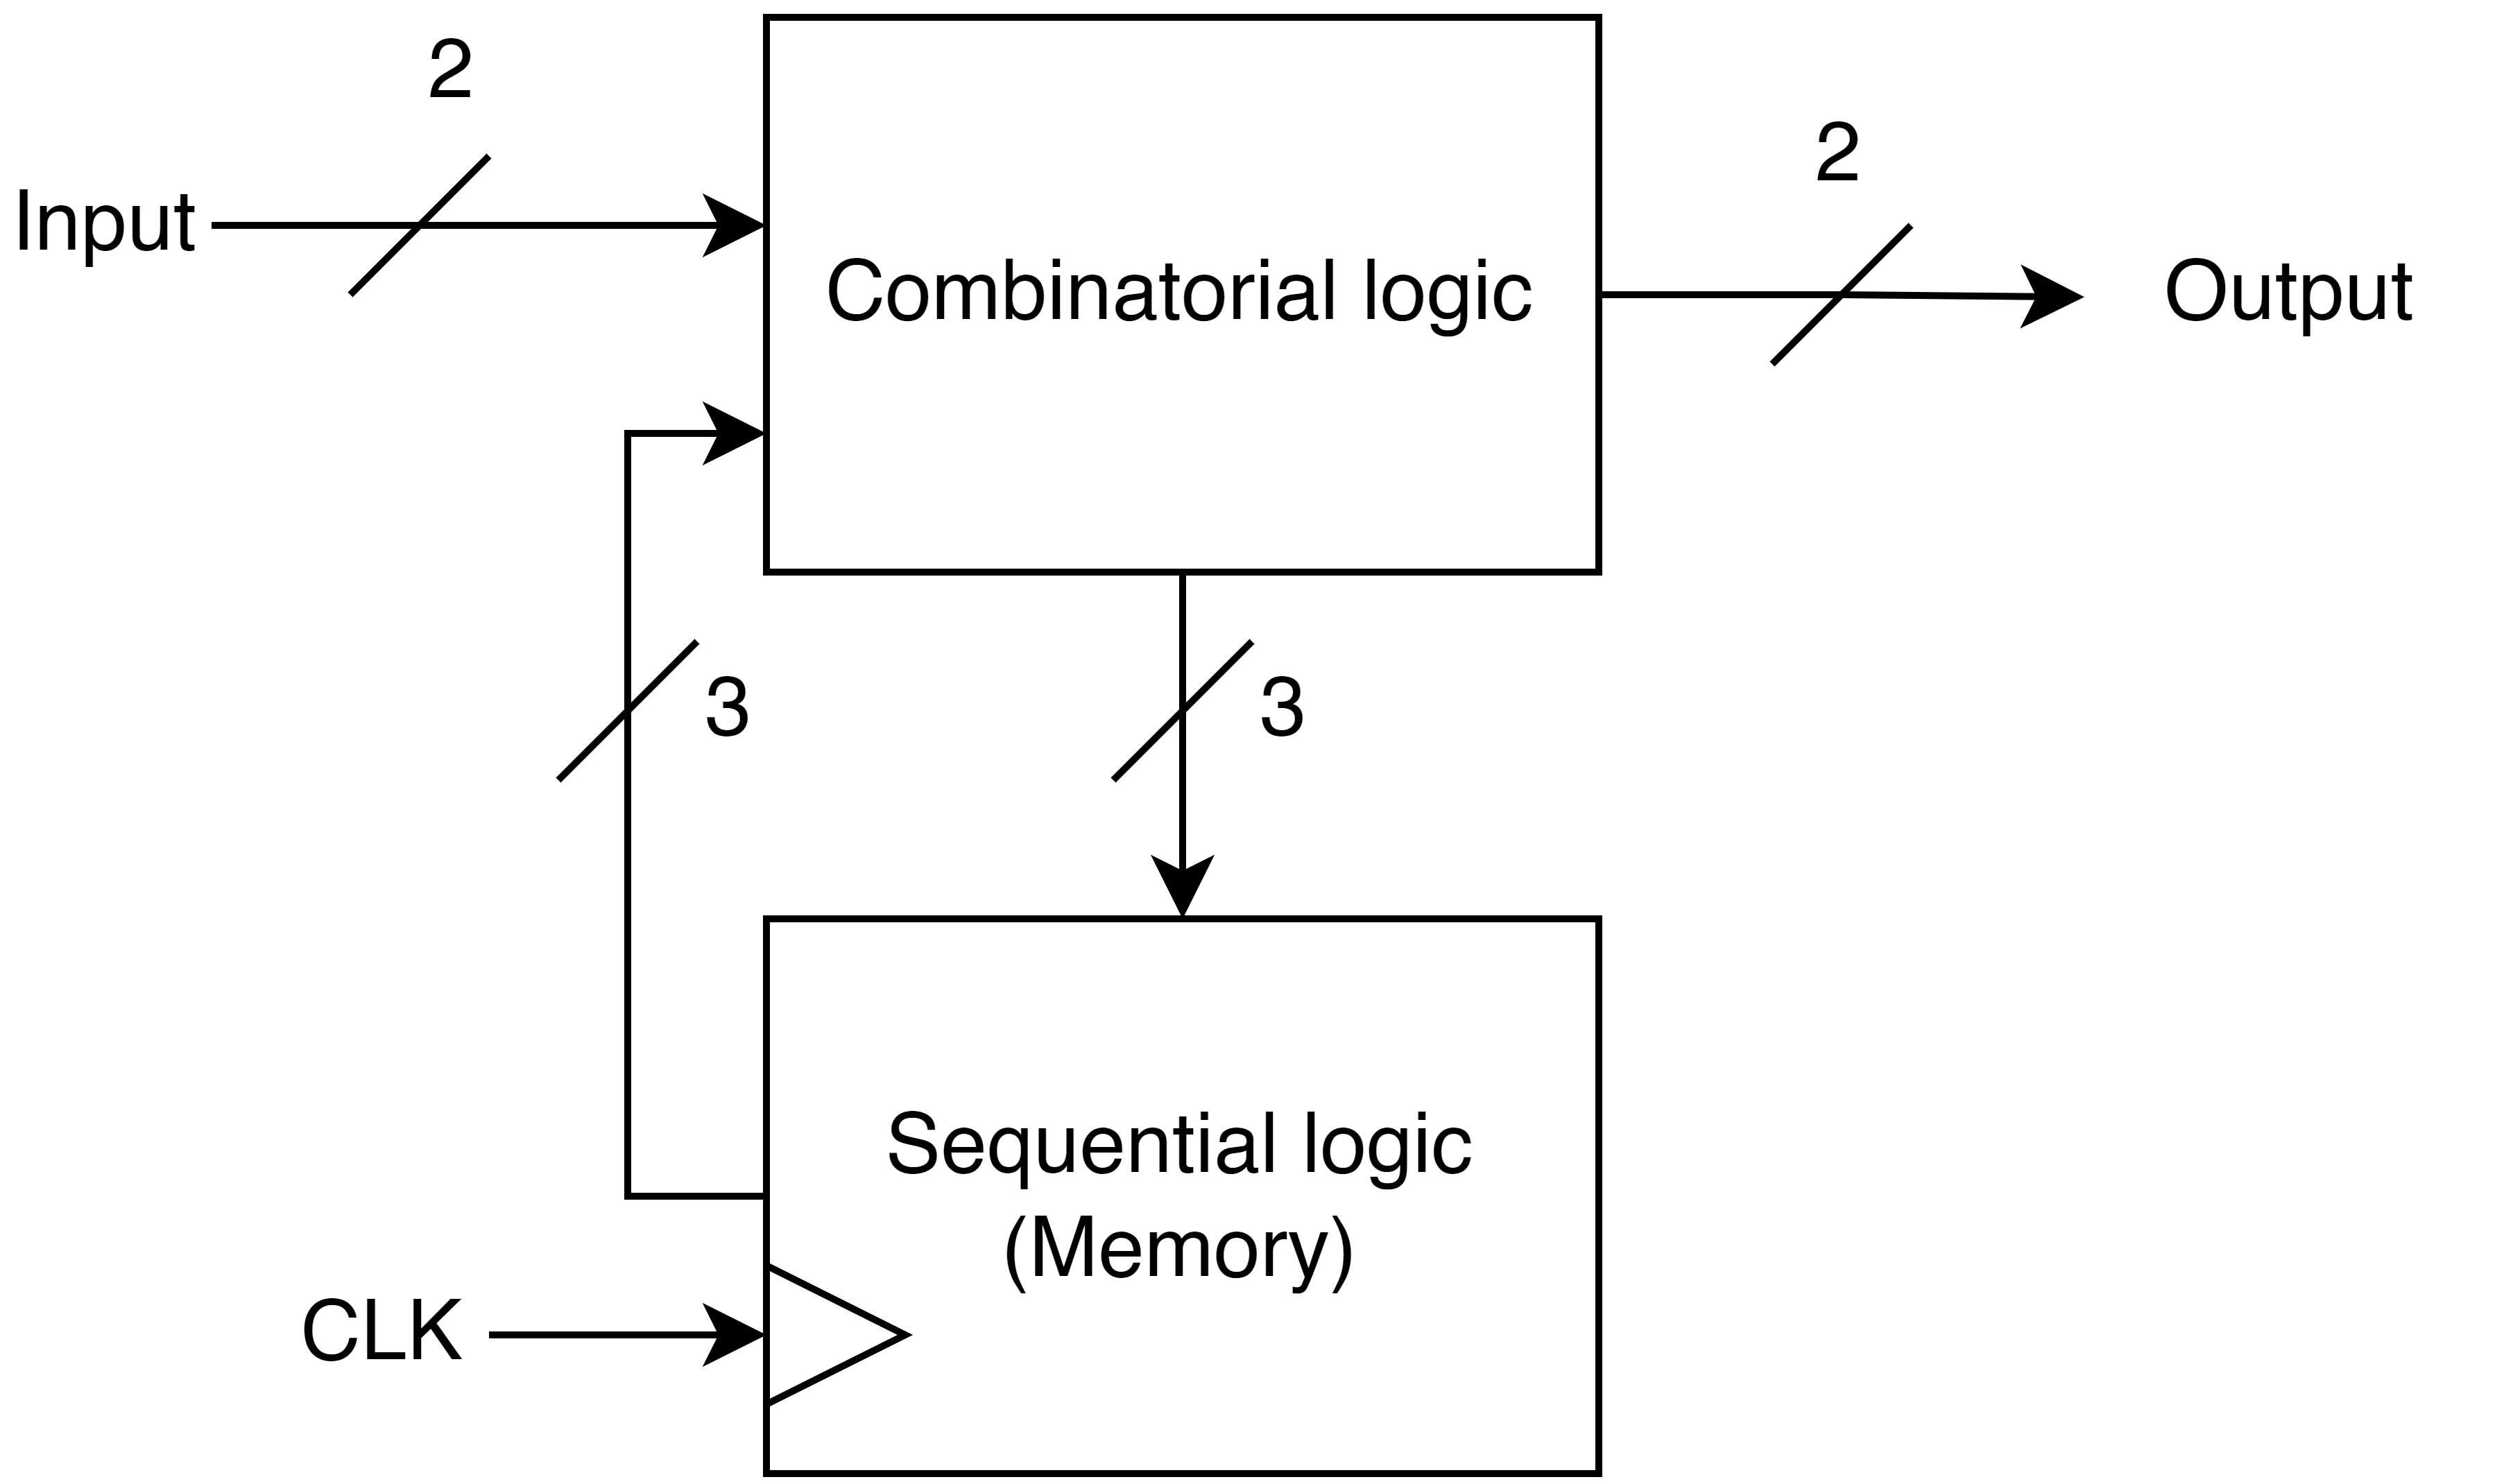
\includegraphics[width=0.6\textwidth]{Figures/FSM_overordnet.drawio.png}
    \caption{FSM general topology diagram}
    \label{fig:fsm_overordnet}
\end{figure}

The current state is from here described by the three signals $C_2$, $C_1$ and $C_0$. The next state is describrd by the three signals $N_2$, $N_1$ and $N_0$.

Figure~\ref{fig:fsm_diagram} and table~\ref{tab:truthtable} show a detailed overview of the wanted functionality of the FSM, describing the relation between inputs, outputs, current state and next state. Transitions for each current state and input is described by arrows, and output is described within each state ($C_2 C_1 C_0$/$O_1 O_0$)

\begin{figure}[H]
    \centering
    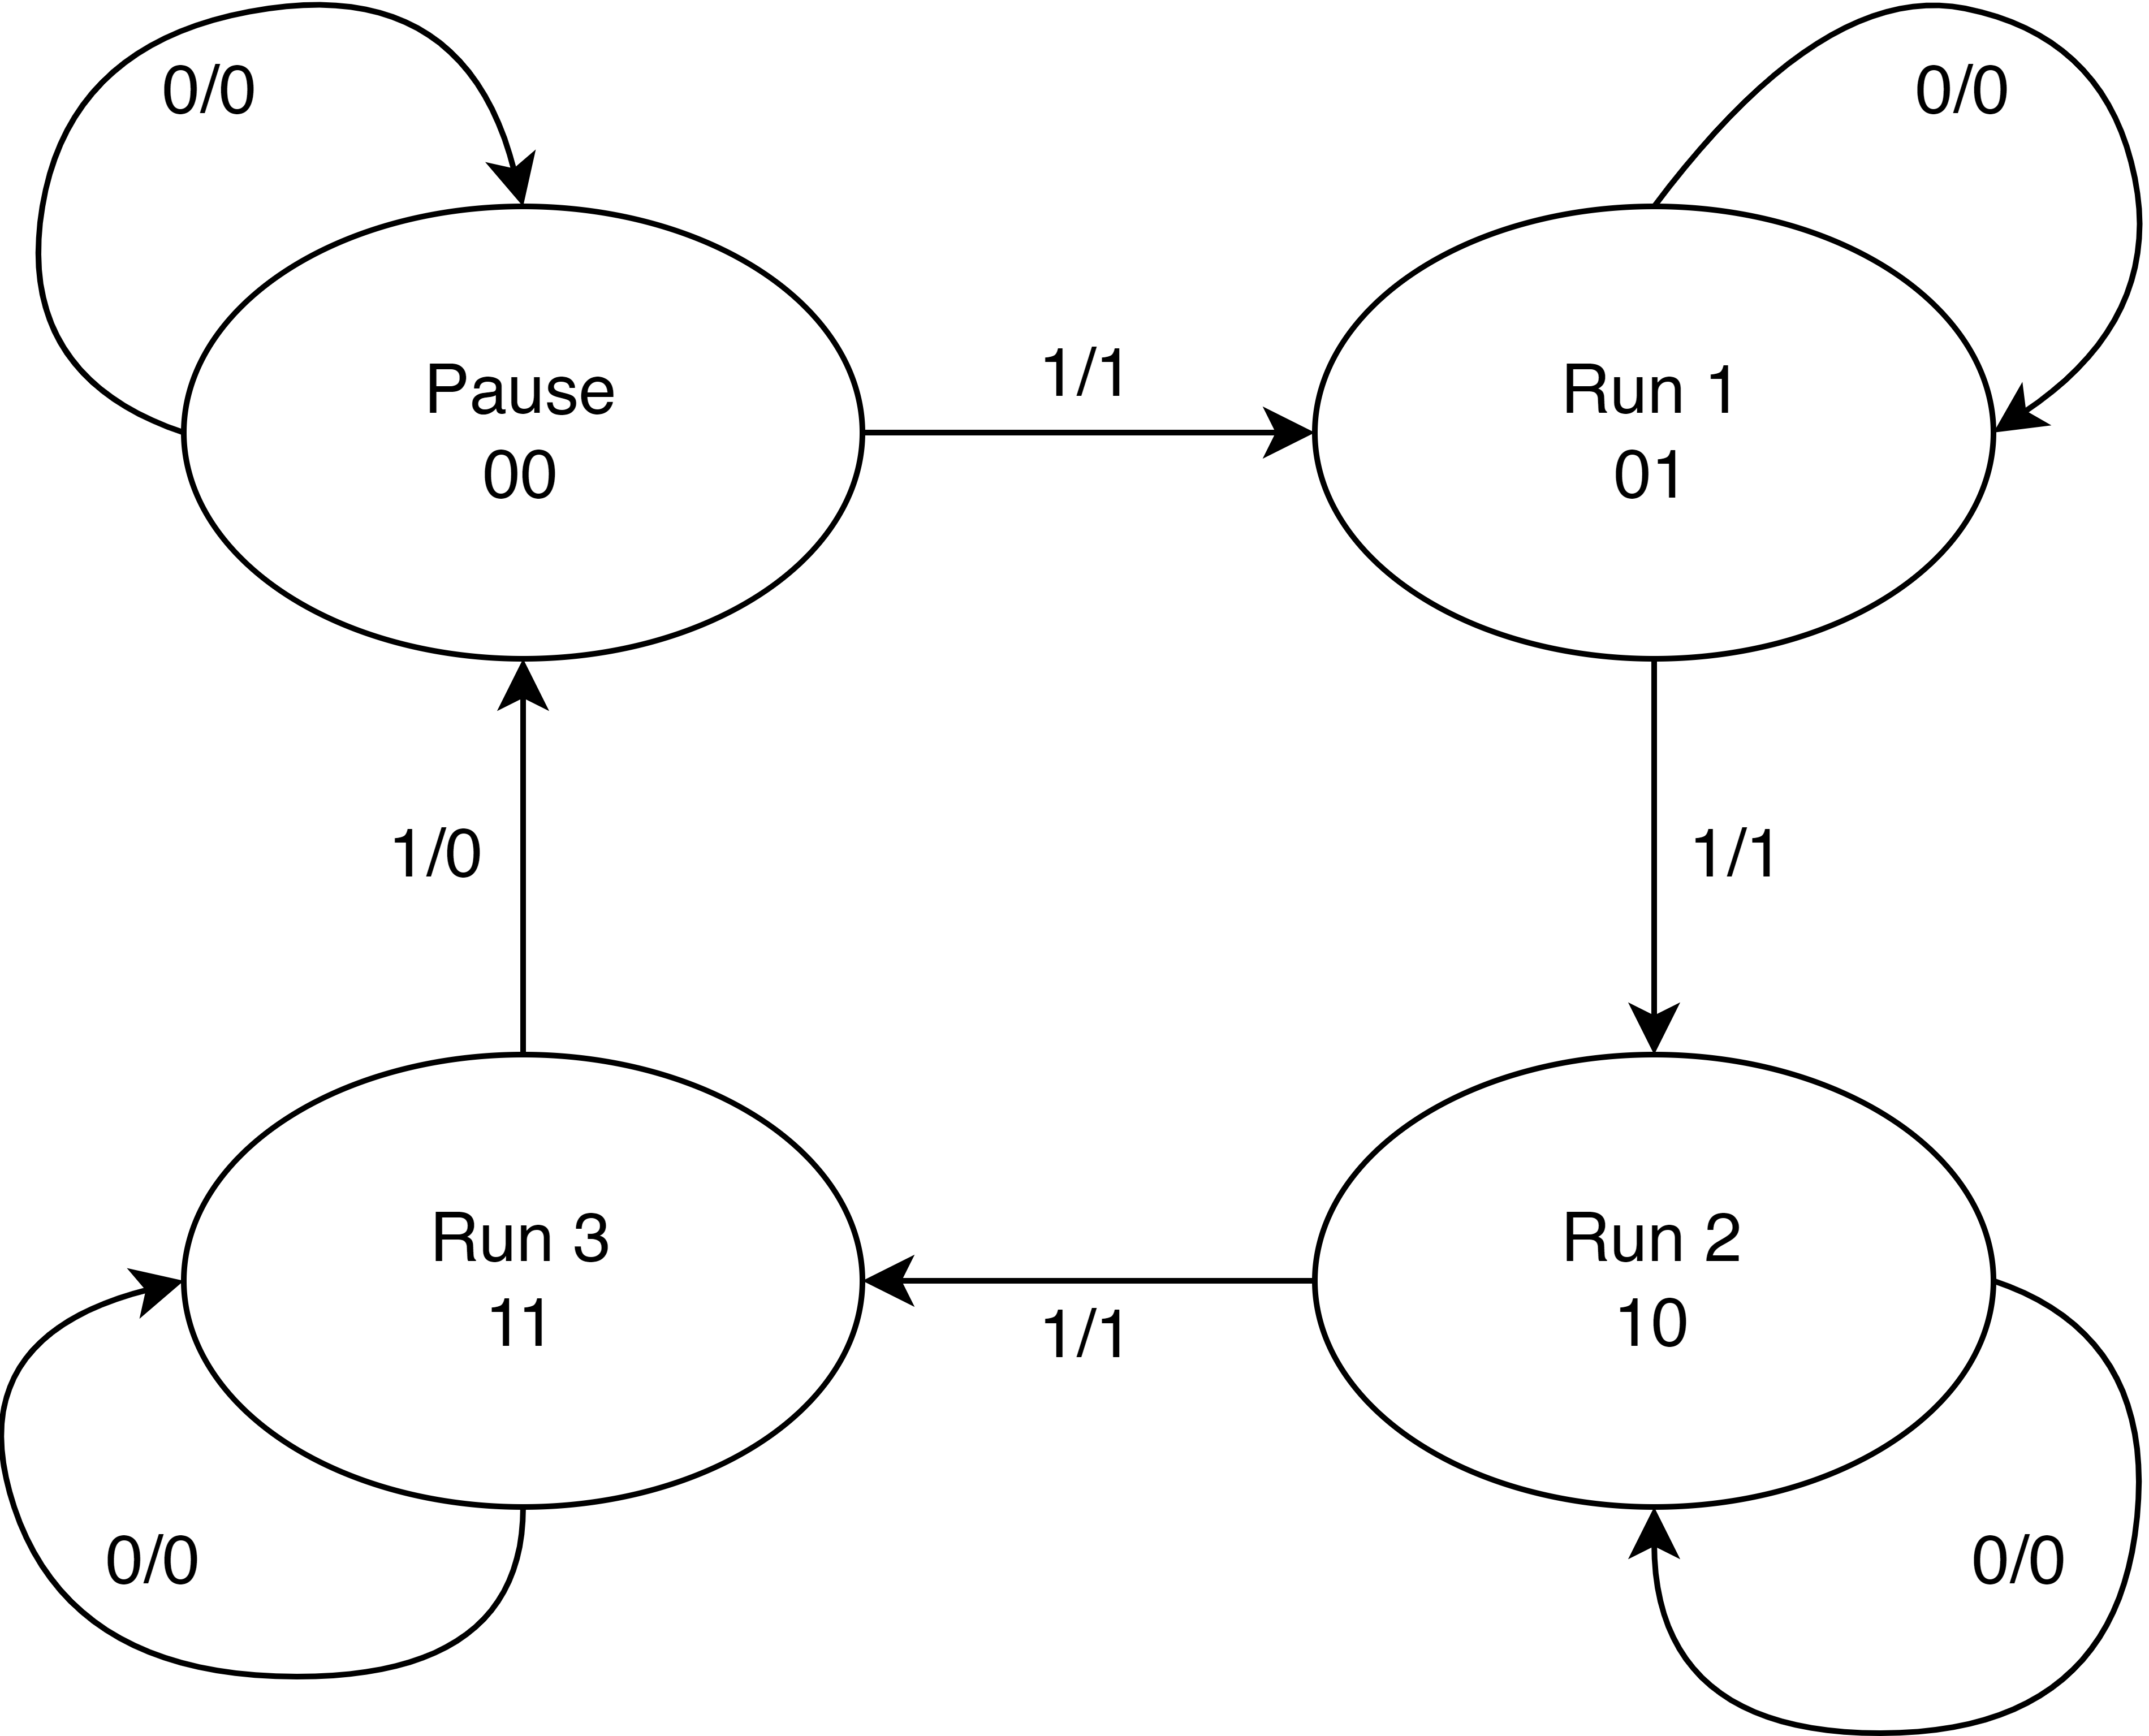
\includegraphics[width=0.8\textwidth]{Figures/FSM-diagram.png}
    \caption{FSM Diagram}
    \label{fig:fsm_diagram}
\end{figure}

\begin{table}[H]
\caption{Truth table for the FSM}
\label{tab:truthtable}
\centering
\begin{tabular}{|l|l|l|l|l|l|l|l|l|l|}
\hline
\rowcolor[HTML]{C0C0C0} 
$C_2$ & $C_1$ & $C_0$ & $I_1$ & $I_0$ & $N_2$ & $N_1$ & $N_0$ & $O_1$ & $O_0$ \\ \hline
0  & 0  & 0  & 0   & 0   & 0  & 0  & 0  & 0   & 0   \\ \hline
0  & 0  & 0  & 0   & 1   & 0  & 0  & 1  & 0   & 0   \\ \hline
0  & 0  & 0  & 1   & 0   & 1  & 1  & 0  & 0   & 0   \\ \hline
0  & 0  & 0  & 1   & 1   & 1  & 1  & 0  & 0   & 0   \\ \hline
0  & 0  & 1  & 0   & 0   & 1  & 0  & 0  & 0   & 1   \\ \hline
0  & 0  & 1  & 0   & 1   & 0  & 1  & 0  & 0   & 1   \\ \hline
0  & 0  & 1  & 1   & 0   & 1  & 1  & 0  & 0   & 1   \\ \hline
0  & 0  & 1  & 1   & 1   & 1  & 1  & 0  & 0   & 1   \\ \hline
0  & 1  & 0  & 0   & 0   & 1  & 0  & 1  & 0   & 1   \\ \hline
0  & 1  & 0  & 0   & 1   & 0  & 1  & 1  & 0   & 1   \\ \hline
0  & 1  & 0  & 1   & 0   & 1  & 1  & 0  & 0   & 1   \\ \hline
0  & 1  & 0  & 1   & 1   & 1  & 1  & 0  & 0   & 1   \\ \hline
0  & 1  & 1  & 0   & 0   & 0  & 0  & 0  & 0   & 1   \\ \hline
0  & 1  & 1  & 0   & 1   & 0  & 0  & 0  & 0   & 1   \\ \hline
0  & 1  & 1  & 1   & 0   & 1  & 1  & 0  & 0   & 1   \\ \hline
0  & 1  & 1  & 1   & 1   & 1  & 1  & 0  & 0   & 1   \\ \hline
1  & 0  & 0  & 0   & 0   & 1  & 0  & 0  & 0   & 0   \\ \hline
1  & 0  & 0  & 0   & 1   & 0  & 1  & 0  & 0   & 0   \\ \hline
1  & 0  & 0  & 1   & 0   & 1  & 1  & 0  & 0   & 0   \\ \hline
1  & 0  & 0  & 1   & 1   & 1  & 1  & 0  & 0   & 0   \\ \hline
1  & 0  & 1  & 0   & 0   & 1  & 0  & 1  & 0   & 0   \\ \hline
1  & 0  & 1  & 0   & 1   & 0  & 1  & 1  & 0   & 0   \\ \hline
1  & 0  & 1  & 1   & 0   & 1  & 1  & 0  & 0   & 0   \\ \hline
1  & 0  & 1  & 1   & 1   & 1  & 1  & 0  & 0   & 0   \\ \hline
1  & 1  & 0  & 0   & 0   & 0  & 0  & 0  & 1   & 0   \\ \hline
1  & 1  & 0  & 0   & 1   & 0  & 0  & 1  & 1   & 0   \\ \hline
1  & 1  & 0  & 1   & 0   & 1  & 1  & 0  & 1   & 0   \\ \hline
1  & 1  & 0  & 1   & 1   & 1  & 1  & 0  & 1   & 0   \\ \hline
\end{tabular}
\end{table}



In this section you should explain what you have done, and how you have done it. The explanations should have enough detail to make a reproduction possible (i.e. it should be possible to do exactly what you have done, and receive the same results, only by doing what you write in this section).


It might be relevant to refer back to a part of theory, as explained in \autoref{subsec:theory_aSubsection}, to explain the design choices you made.

\subsection{Must include}
The method section MUST INCLUDE:
\begin{itemize}
    \item One or more illustrations showing your circuit. As a minimum you must include one figure of the circuit at the logic gate level, and one of what you implemented at transistor level in AIMSpice.
    \item Figure showing the state diagram for your final state machine (FSM).
    \item Explanations of design choices you made when creating the circuit.
    \item Explanations of the simulations you did (not the results, just how they were done).
\end{itemize}